\section{Irreversible Thermodynamics}

When we talked about physical quantities we mentioned also the presence of a part of them called transport properties, where was sad that they appeared in the study of irreversible phenomena. Such phenomena are can be thought simply as the kinetic evolution of the system in time when it's out of equilibrium. In fact, a system where transport of matter, energy or momenta is present inside it can't be in equilibrium and can be seen by some simple examples. Take two thermal reservoirs at temperatures $T$ and $T + \Delta T$ that are in contact through a cave. A thermal current $I_Q$ will be present between the two, and we know that a variation of entropy is generated in both of them as
\begin{align}
    &\dv{S_1}{t} = -\frac{I_Q}{T + \Delta T}, &\dv{S_2}{t} = \frac{I_Q}{T}.
\end{align}
Thus, we can write down the total variation of entropy inside the system by taking the sum of the two and seeing how
\begin{equation}
    \dv{S}{t} \approx \frac{I_Q}{T}\frac{\Delta T}{T} > 0,
\end{equation}
meaning that the process is irreversible since a variation of entropy is created and the system is not in equilibrium as it happens. Also, this is only an example, but every single process that involve a current posses the same property, like charge current $I_q$. The power dissipated in the environment through Jaul effect, in fact, generates entropy since we have
\begin{align}
    &P = \Delta V I_q, & \dv{S}{t} = \frac{P}{T} = \frac{\Delta V}{T}I_q.
\end{align}
Where we can see how in both cases the entropy increase has a form composed by the product of a \textbf{flux}, like $I_Q$ or $I_q$, by a gradient, which usually represent the \textbf{driving force} that in these cases were the electric force $\Delta V$ and the thermal gradient $\Delta T$.

Therefore, if we aim at describing the kinetic properties of matter and how atoms move inside it, we will need to restate thermodynamics in order to account also for irreversible process.

\subsection{Entropy production}

The first thing we need to do is understand how entropy is created to its core, and to do it we are going to make a general construction to tackle the problem using already known results. Basically we want to imagine that every non equilibrium system can still be seen as multiple ones that are in local equilibrium that interacting altogether locally generates entropy over time. Basically we are assuming something that we are going to call \textbf{local thermodynamic equilibrium} that we are going to formally define in the following way.
\dfn{Local thermodynamic equilibrium}
{
    A general system is in local thermodynamic equilibrium if it can be divided in a series of smaller subsystems with thermodynamics fully defined by the values of the thermodynamic potential within the cell. Meaning that the generalized first principle is valid within the subsystem as
    \begin{equation}
        \label{eq:LocTheEqui}
        T\dd s = \dd u - \psi_i\dd \xi_i,
    \end{equation}
    where $\psi_i$ are the thermodynamic potentials, and $\xi_i$ are their conjugate responses.
}
\noindent
Notice how small letters, like $s$, $u$, were used in the definition since we are focussing on densities and not on the total properties in the system. Also, notice how we are using Einstein convention.

This principle will be our key to use known results in the study of the more complex behaviors of irreversible processes. In particular, by assuming it on a system we can easily obtain a first result inside a general system as follows.
\thm{General continuity equation}
{
    Inside a system in local thermodynamic equilibrium, where non-zero local entropy production $\dot{\sigma}$ is present the following continuity relation for the entropy is valid
    \begin{equation}
        \label{eq:ContEquEntropy}
        \pdv{s}{t} = \dot{\sigma} - \grad\vdot\vb{J}_s.
    \end{equation}
}
\pf{Proof}
{
    The proof it's really easy, basically from classical mechanics we know how a conserved quantity $c$ needs to respect the continuity equation
    \begin{equation}
        \pdv{c}{t} = - \grad\vdot\vb{J}_c,
    \end{equation}
    which tells us that the variation of $c$ are given by the quantity that was entering minus the one going out. In the case of entropy here we have that in it is also being created by the system \textbf{locally}, assumption given by the local equilibrium. Thus, the variation in time of the entropy must account also for $\dot{\sigma}$ giving \eqref{eq:ContEquEntropy}.
}
\noindent
Therefore, we are starting to account for the presence of source of entropy inside our system that can change the behavior of the whole solid, but one may ask what those sources are. We have already seen them in the previous discussion, in reality, seeing how currents are able to generate variations of entropy locally and that can be set on a general ground in the following way.
\thm{Current generates entropy}
{
    Inside a system in local thermodynamic equilibrium the variation of entropy is generated through the presence of current inside a system, where the local generation of entropy $\dot{\sigma}$ is given by
    \begin{equation}
        \label{eq:EntroProduct}
        T\dot{\sigma} = -\frac{\vb{J}_Q}{T}\vdot\grad T - \vb{J}_i\vdot\grad\xi_i.
    \end{equation}
}
\pf{Proof}
{
    We can start by writing down a form for the variation of entropy in time by using \eqref{eq:LocTheEqui}
    \begin{equation}
        \pdv{s}{t} = \frac{1}{T}\pdv{u}{t} - \frac{1}{T}\psi_i\pdv{\xi_i}{t}.
    \end{equation}
    Then, we can use the normal continuity equations on the energy densities and on the conjugates responses having that
    \begin{equation}
        \pdv{s}{t} = -\frac{1}{T}\grad\vdot\vb{J}_u + \frac{1}{T}\psi_i\grad\vdot\vb{J}_i,
    \end{equation}
    with $\vb{J}_i$ the flux related to quantity $\xi_i$. Then we can use the algebraic identity $A\grad\vdot \vb{B} = \grad(A\vb{B}) - \vb{B}\vdot\grad A$ to obtain the following form
    \begin{equation}
        \label{eq:intermediateCGE}
        \pdv{s}{t} = \vb{J}_u\vdot\grad\left( \frac{1}{T} \right) - \vb{J}_i\vdot\grad\left( \frac{\psi_i}{T} \right) - \grad\vdot\left( \frac{\vb{J}_u - \psi_i\vb{J}_i}{T} \right).
    \end{equation}
    We can then use once again \eqref{eq:LocTheEqui} and taking its time derivative to notice how the last term is simply $\grad\vdot\vb{J}_s$, so that by substituting \eqref{eq:intermediateCGE} inside \eqref{eq:ContEquEntropy} we can find out that
    \begin{equation}
        \dot{\sigma} = \vb{J}_u\vdot\grad\left( \frac{1}{T} \right) - \vb{J}_i\vdot\grad\left( \frac{\psi_i}{T} \right).
    \end{equation}
    Nevertheless, we can use the general first principle of thermodynamics to rewrite the flux of energy in a form that simplify the expression as
    \begin{align}
        &\dd u = \delta Q + \psi_i \dd \xi_i, &\vb{J}_u = \vb{J}_Q + \psi_i\vb{J}_i,
    \end{align}
    that inserted in the previous result allow us to arrive at the form
    \begin{equation}
        \dot{\sigma} = \vb{J}_Q\vdot\grad\left( \frac{1}{T} \right) - \frac{\vb{J}_i}{T}\vdot\grad\psi_i.
    \end{equation}
    Then by using the known relation $\grad 1/T = -T^{-2}\grad T$ we obtain the wanted result.
}
\noindent
Therefore, the presence of a current means that an irreversible process is happening and vice versa. For this reason will be useful to see some examples of possible currents that will probably appear in our studies like
\begin{align}
    &\text{Heat}, \hspace{2cm} \vb{J}_Q, \hspace{2cm} -\frac{\grad T}{T}, \hspace{2cm} \vb{J}_Q = -\kappa \grad T;\\
    &\text{Charge}, \hspace{1.6cm} \vb{J}_q, \hspace{2.1cm} -\grad \phi, \hspace{2cm} \vb{J}_q = -\rho^{-1} \grad \phi;\\
    &\text{Matter}, \hspace{1.7cm} \vb{J}_i, \hspace{2.2cm} -\grad \mu, \hspace{2cm} \vb{J}_i = -c_i M_i \grad \mu.
\end{align}
Where along with the general known forms for the conjugated flux also the driving force was reported, and is possible to see how the latter is always a gradient so that the product of flux and force generate an \textbf{energy density dissipation}. Also, the relations known that connect the two is always linear relation with a transport property, like $\kappa$, $\rho$ or $c_i M_i$, that connects force and response.

The result obtained is actually really great one that allows us to understand how the variation of entropy is effectively created inside a system. Nevertheless, something else can be actually sad about the variation of entropy. In particular, from second principle we know that in general the total entropy of the system always increase, so that is possible to have situations where the local entropy decrease but the one of the environment compensate having a total that is positive. Still, this situation can be really complex to tackle in a general situation so that we are going to make a really important assumption in order to make things easier.
\dfn{Postulate of irreversible thermodynamic}
{
    In proximity of equilibrium, the local rate of entropy production is non-negative
    \begin{equation}
        \dot{\sigma} \ge 0.
    \end{equation}
}
\noindent
Basically, we are ruling out the possibility of even having local increase of the order of the system if we are in a situation close to equilibrium. That is actually interesting since we can easily apply it to \eqref{eq:EntroProduct} to see that
\begin{equation}
    T\dot{\sigma} = -\vb{J}_Q\vdot\frac{\grad T}{T} = \frac{\kappa \laplacian T}{T} \ge 0,
\end{equation}
meaning that the value of $\kappa$ needs to be positive near equilibrium. This applies on every transport property, having that $\rho$ and all $M_i$ needs to be positive near equilibrium.

\subsection{Linear irreversible thermodynamics}

Now, we have seen how as in equilibrium thermodynamic we have generalized forces connected to conjugated responses here we have driving forces that are related to flows. Therefore, we might want to follow the same reasoning and find out a constitutive relation between the driving forces and the fluxes. In particular, recalling the general form obtained for the static physical quantities we can imagine that a flux $\vb{J}$ do not only depend on it's driving force but all of them give a contribution, having in general
\begin{align}
    &\vb{J} = \vb{J}(\vb{F}), &\vb{F} = \left(\frac{\grad T}{T}, \grad \phi, \dots\right).
\end{align}
Then, we can make a linear approximation for this relation since we have already seen how some known forms for the fluxes linearly depend on the conjugated driving forces. Therefore, we can simply assume that a form for the general relation between the two quantities is the following
\begin{equation}
    J_\alpha = \pdv{J_\alpha}{F_\beta}F_\beta = \mathcal{L}_{\alpha\beta}F_\beta.
\end{equation}
Defining, so, a general matrix $\vb*{\mathcal{L}}$ that contains all the information on the transport properties of the system.

Also, we can now study this new matrix and see their properties in a way analogous to the one seen for the $\mathcal{K}$ matrix seen for static properties. In particular the first thing that we can say is the following.
\thm{Positivity of $\mathcal{L}$}
{
    In a near equilibrium situation the $\mathcal{L}$ matrix is a positive one.
}
\pf{Proof}
{
    We can use the principle of irreversible thermodynamic to write down the following thing
    \begin{equation}
        T\dot{\sigma} = J_\alpha F_\alpha = \mathcal{L}_{\alpha\beta}F_\beta F_\alpha \ge 0,
    \end{equation}
    which is valid for every value of $F_\alpha$ and $F_\beta$ meaning that $\vb*{\mathcal{L}}$ is positive.
}
\noindent
Still, the most important relations, as we have seen in the first part, concern the symmetry properties of the matrix, which are similar to the one of $\mathcal{K}$ since the following result can be proven formally.
\thm{Onsager’s symmetry principle}
{
    The $\mathcal{L}$ matrix is a symmetric one, and therefore the following is true
    \begin{equation}
        \mathcal{L}_{\alpha\beta} = \mathcal{L}_{\beta\alpha}.
    \end{equation}
}
\pf{Proof}
{
    The proof is complex and goes microscopically imposing the detailed balance on the fluxes near equilibrium. We haven't seen it during the course, and so I'm not going put it here for now.
}

\noindent
The same symmetric properties that is often present inside important physics matrices, if not all of them, is found out. We can also have a look at how this property can also be restated as
\begin{equation}
    \pdv{J_\alpha}{F_\beta} = \pdv{J_\beta}{F_\alpha},
\end{equation} 
which have a form similar to Maxwell's relations seen in equilibrium thermodynamics. Also, as we have seen for the $\mathcal{K}$ matrix we can see how various blocks are presen,t and we can have a little look at them really quickly

\paragraph{\bf k thermal conductivity, $\vb*{T}_S(2)$.} Relates temperature gradient and heat current, and from symmetry properties it's easy to see how
\begin{equation}
    k_{\alpha\beta} = k_{\beta\alpha}.
\end{equation}

\paragraph{$\vb*{\sigma}$ \bf electrical conductivity, $\vb*{T}_S(2)$.} Relates electric potential and charge current, its inverse is the resistivity and also this is symmetric.

\paragraph{$\vb*{\beta}$, $\vb*{\beta}'$ \bf thermoelectric cross effects.} Off diagonal term that relates the electric potential with heat current and temperature gradient with charge current. It's easy to see how from $\mathcal{L}$ symmetry one can find out that since are off diagonal terms
\begin{equation}
    \label{eq:ThermoeTensorProp}
    \beta_{ij} = \beta'_{ji}.
\end{equation}

\paragraph{\bf $\vb{D}_i$ diffusivity, $\vb*{T}_S(2)$.} It's the more general way of writing down $c_i M_i$ term for matter transport appearing in Fick's law, the real way of writing down $\vb{J}_i$. The appendix $i$ describe the type of component is getting transported, and $D_i$ has the same symmetry properties of the others diagonal terms.

\subsection{Thermoelectric materials}

To make an example of the use irreversible thermodynamic theory can have we can look at the properties of thermoelectric materials. The latter are systems that are able to generate potential gradients due to the presence of a thermal one, and vice versa. Basically, thermoelectric materials are systems that posses a non-zero $\beta$ component inside the $\mathcal{L}$ matrix, so that the constitutive relations of the heat and charge flux becomes coupled equations with
\begin{align}
    \label{eq:ConstThermoe}
    &\vb{J}_Q = -k\grad T - \beta'\grad \phi, &\vb{J}_q = -\frac{\beta}{T}\grad T - \sigma\grad \phi.
\end{align}
This shows how the movement of the microscopic elements inside the material is intrinsically related to the flux of both charge and energy. In fact, the electrons are the main charge and heat transport carrier inside matter, meaning that a movement of heat inside a material often means that also charge is being transported. Nevertheless, we want to focus on the relation between the driving forces in this case and in particular in an equilibrium situation where the fluxes are zero meaning that $\vb{J}_q = 0$ and
\begin{align}
    &\grad \phi = -S\grad T, &S = \frac{\rho\beta}{T}.
\end{align}
A linear relation between the two appears giving rise to the \textbf{Seebeck effect}, a really important phenomenon that tells us that a variation of temperature can generate a potential with an intensity dependent on $S$, called \textbf{thermopower}. This is a really important information that is used a lot in technological applications to measure temperature using instruments called thermocouples. Still, this is not the only interesting thing we can say about equations \eqref{eq:ConstThermoe} since another situation can appear where, at non equilibrium, we have both transport of charge and heat but with a constant temperature in the system. This condition is called \textbf{Peltier effect} and describes how the presence of electrons moving in the system due to a potential gradient also generates a heat current even if no heat gradient is present in the material. Therefore, by placing $\grad T$ to be null we can see how
\begin{align}
    &\vb{J}_Q = \Pi\vb{J}_q, &\Pi = \beta'\rho,
\end{align}
where we can also see how a relation between $\Pi$ and $S$ is present. In fact, by using that $\rho$ is a symmetric tensor and \eqref{eq:ThermoeTensorProp} we can easily see that
\begin{equation}
    \Pi_{ij} = TS_{ij},
\end{equation}
which is an interesting relation first proven by lord Kelvin. Thus, all thermoelectric properties can be described by the value of $S$, which can be found out using particular transport models. We have, obviously, not seen those since can be really complex, especially if a semi-classical one is used, giving out directly the final results for \textbf{metal} and \textbf{semiconductor} respectively
\begin{align}
    &S_{met} \approx \left( \frac{k_B}{e} \right)\frac{k_BT}{E_F}, &S_{sco} \approx \left( \frac{k_B}{e} \right)\frac{E_g}{k_BT}.
\end{align}
Where, we can understand that the constant in front gives out the order of magnitude for the value of $S$, which is $k_B/e \approx \SI{87}{\micro\volt/\kelvin}$. Also, we can see how metals and semiconductors differ since $S$ is much smaller in the formers than the others since usually $E_F \gg k_BT$ at room temperature, while $E_g \approx k_BT$. In addition, semiconductors can display both negative and positive thermopower, for electron and hole conduction respectively, so that in general the real value of the coefficient is a weighted mean of the two
\begin{equation}
    S\approx \frac{\sigma_nS_n + \sigma_pS_p}{\sigma_n + \sigma_p}.
\end{equation}
Where the subscript $n$ is for electrons while $p$ is for holes.

Seebeck and Peltier effects are extensively used for technological applications of several kinds. For example, the Peltier effect can be used to create efficient and simple refrigeration mechanisms where, by using an electric current you can induce a heat one between two objects that will then cool down. Also, similarly you can use heat to generate $\vb{J}_Q$ that induces electrical transport to power other apparatus. This two type of applications are described schematically in \figref{fig:ThermoAppl}, and are impactful in a lot of fields like spacecraft engineering where Radioisotope Thermoelectric Generators(RTG) are widely used.
\begin{figure}[t]
    \centering
    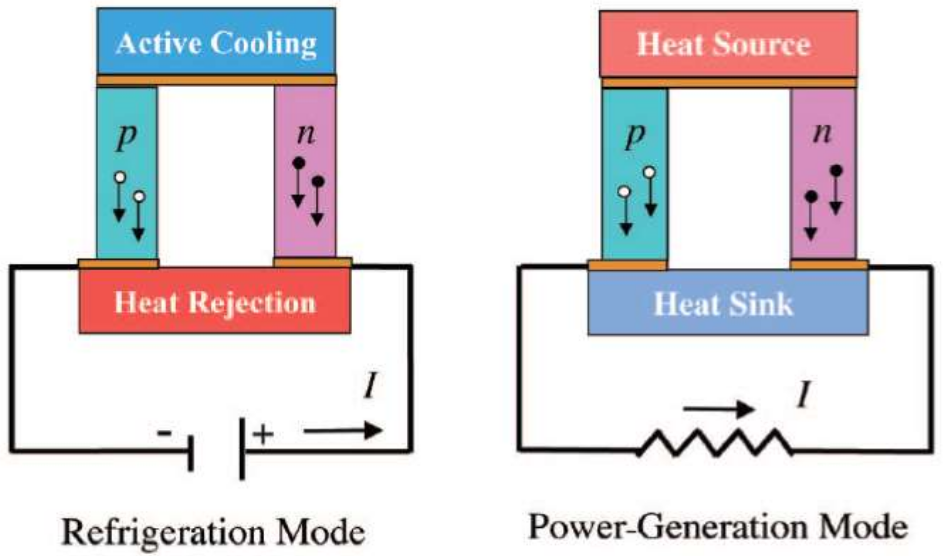
\includegraphics[width=0.8\textwidth]{Immagini/ThermoAppl.png}
    \caption
    {
        Diagram of a Peltier thermoelectric couple made of an n-type and a p-type thermoelectric material. Refrigeration and power generation modes are possible, depending on the configuration.
    }
    \label{fig:ThermoAppl}
\end{figure}
Such devices bring a lot of advantages in genera, like the fact that no moving parts are present giving: high reliability, no noise, no vibration or torque. Also, they are usually highly resistant to radiations and can be miniaturized. Therefore, it's of our interest to understand the characteristic that a material needs to have in order for it to be a good one to create such instruments. Thus, a figure of merit for thermoelectric materials is defined in the following way
\begin{equation}
    \label{eq:ZT}
    ZT \equiv \frac{S^2\sigma T}{\kappa},
\end{equation}
where $\sigma$ is the electrical conductivity, while $\kappa$ is the thermal conductivity. Still this is the definition for a device made of a single material, while it's possible to have one made out of both n and p type conductors do that a more general definition that takes that into account would be
\begin{equation}
    ZT \equiv \frac{\left( S_n - S_p \right)^2T}{\sqrt{\left( \rho_n\kappa_n \right)^2 + \left( \rho_p\kappa_p \right)^2}}.
\end{equation}
Using this definition we can also see the efficiency of the machince that we are going to build by using the following relation
\begin{equation}
    \eta = \frac{T_H - T_C}{T_H}\left( \frac{\sqrt{1 + ZT_M} - 1}{\sqrt{1 + ZT_M} + T_C/T_H} \right),
\end{equation}
where $T_H$, $T_C$ and $T_M$ are hot, cold and mean temperature in the system. Where we can see how the term in front has the form of the Carnot efficiency, meaning that the two are related and that $\eta \to \eta_{c}$ for $ZT \to \infty$. Therefore, we are looking for materials that posses $ZT$ high as possible in order to increase our efficiency closer as we can to the thermodynamic limit.

In order to maximize the value of $ZT$ we can look at \eqref{eq:ZT} and see how the best thing is to have low thermal conductivity but greate electrical one. Still this is not so easy to achive since we know that two contributions are present inside $\kappa$, electrical and phononic one, and the former is related to $\sigma$ by the \textbf{Wiedenmann-Franz law}
\begin{align}
    &\kappa = \kappa_E + \kappa_P, &\kappa_E = L\sigma T,
\end{align}  
where $L$ is a constant called Lorentz number. Therefore, the best we can do is to get $\kappa_P$ as low as possible meaning that we aim at having the smallest phonon free path since we know that
\begin{equation}
    \kappa_P = \frac{1}{3}v_sC\lambda_{P},
\end{equation}
where $v_s$ is the velocity of sound. In general, we can imagine that a really low value of $\lambda_P$ would be as the interatomic distance so that an estimate of $\kappa_P$ would be \SI{0.25}{W\metre^{-1}\kelvin^{-1}}. But, even if $\kappa_P$ would be really low the thermopower needed in order to achieve a value of $ZT = 1$ is really high. In particular, by using an idea zero phonon conductivity model we would obtain $S = \sqrt{L}$ which means \SI{160}{\micro\volt\kelvin^{-1}}. In this optic the better type of material we can aim for are semiconductors with narrow-bandgap which posses high mobility, in order to maximize the value of $S$ by the fact that hole and electron coefficients add up.